\documentclass{article}
\usepackage[utf8]{inputenc}
\usepackage[T1]{fontenc}
\usepackage[danish, english]{babel}
\usepackage[margin=1in]{geometry}
\usepackage{enumitem}
\setlist[enumerate]{itemsep=-1mm}

\usepackage{graphicx}
\usepackage{caption}
\usepackage[textfont=normalfont,singlelinecheck=off,justification=raggedright]{caption}
\addto\captionsenglish{
	\renewcommand{\contentsname}
	{Indholdsfortegnelse}
}
\usepackage{gensymb}
\newcommand{\norm}[1]{\left\lVert#1\right\rVert}
\usepackage{wrapfig}
\usepackage{float}
\usepackage{indentfirst}
\usepackage{flafter}
\usepackage{grffile}
\usepackage{tcolorbox}
\usepackage{hyperref}

\usepackage{amsmath, amsfonts, amssymb}
\setlength\parindent{0pt}

\usepackage{systeme}
\setlength{\voffset}{-0.6in}

\usepackage[utf8]{inputenc}
\usepackage[danish]{babel}
\usepackage{graphicx}
\usepackage{float}
\title{Praktisk programering - Homeworks}

\begin{document}

\maketitle
\begin{center}
	Simon S. Villadsen, 201804389\
\end{center}
	My student id ends with 89 so $89 \equiv 20\  (\operatorname{mod}\ 23)$. The Akima spline interpolation is implemented in subsection \ref{akima}.
\section{Homeworks}
\subsection{Jacobi elimination}
\begin{table}[H]\centering
	\begin{tabular}{|c|}
		\hline
		Methods\\\hline
		\texttt{timesJ}, \texttt{Jtimes}, \texttt{jacobi\_cyclic} in \texttt{jacobi.cs};
		 \texttt{getrandomsymmetric} in \texttt{matrix.cs};\\
		  \texttt{test\_jmd}, \texttt{hydrogen\_jmd} in \texttt{Program.cs};
		   \texttt{plot\_hydrogen\_eigens} in \texttt{Form.cs}; \\
		\hline
	\end{tabular}
\end{table}
Really a given Jacobi matrix $J(p, q)$ can be defined as the identity matrix except for four coordinates $ij\in \{pq, qp, pp, qq\}$ [0]. Let us take a look on the defintion of the matrix product $P=AJ$
\begin{equation}
	P_{ij} = \sum _{k= 0}^n A_{ik}J_{kj}
\end{equation}
So for a given coloumn $j$, $P_{ij}$ only differ from $A_{i, j}$ if $j = p$ or $j = q$. We basically only need to calculate the product along these two colomuns which is done in $\mathcal{O}(n)$ time. The conclusion is similar when computing $JA$. 
\begin{figure}[H]
	\centering
	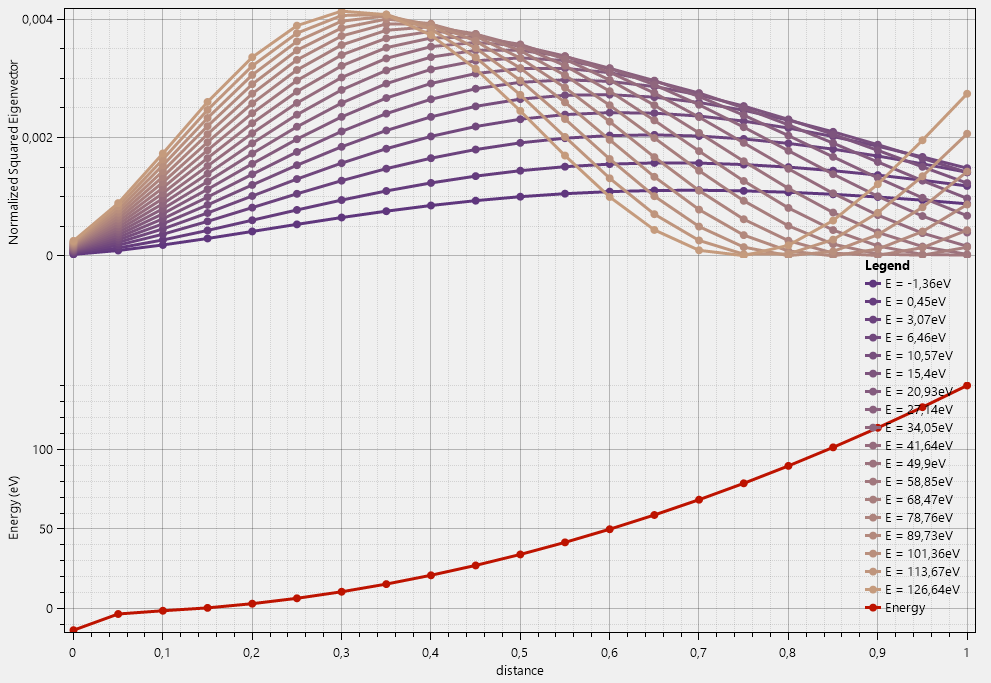
\includegraphics[width=.62\textwidth]{hydrogen_plot.png}
	\caption{Hydrogen eigenvalue and -vector plot, with $dr = 0.05$ and $r_{\mathrm{max}} = 20$.}
\end{figure}

For the schödinger equation we solve the eigenvalue equation $\mathbf{H}f = \epsilon f$, by diagonalising $\mathbf{H} = VDV^T$. The eigenvalues lie along the diagonal of $D$ and the eigenvectors are the coloumn vectors of $V$. We get the lowest and largest energy state values as where we set $dr = 0.1$ and $r_{\mathrm{max}} = 20$. 
{\small
\begin{align}
	-0.49875621120889385\mathrm{\ Hatree} * 27.211386245988\  \frac{\mathrm{eV}}{\mathrm{Hatree}} = -13.5718\ \mathrm{eV}\\
	199,89946101554284\mathrm{\ Hatree} * 27.211386245988\  \frac{\mathrm{eV}}{\mathrm{Hatree}} = 5.43954\ \mathrm{keV}.
\end{align}}%


\subsection{Least Squared method}
\begin{table}[H]\centering
	\begin{tabular}{|c|}
		\hline
		Methods\\\hline
		\texttt{QR\_leastsq\_fit} in \texttt{leastsq.cs}; \texttt{radioactivity\_leastsqs} in \texttt{Form.cs};
		\\
		\texttt{QR\_decomposition}, \texttt{solve\_uppertriangular\_equation}, \texttt{leastsq\_matrix} in \texttt{matrix.cs}; \\
		\hline
	\end{tabular}
\end{table}
\begin{figure}[H]
	\centering
	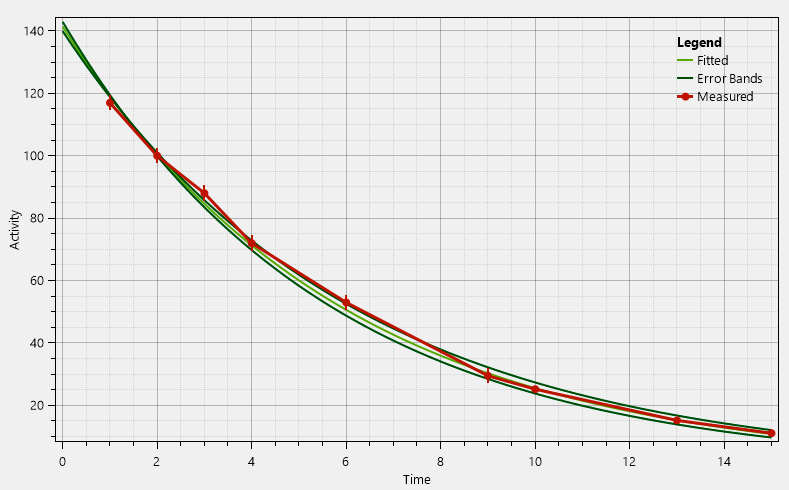
\includegraphics[width=.7\textwidth]{radioactivity_fit.png}
	\caption{Least square QR-decomposition method for radioactivity data for $^{224}\mathrm{Ra}$. The fitted line is the function $a\exp(-\lambda t)$, where $a = 141,45$ and $\lambda = 0,1712\ \mathrm{day}^{-1}$. The atom's half life is $\tau = \frac{\ln 2}{\lambda} =4.05\ \mathrm{days}$. The modern day half life value is $3.6\ \mathrm{days}$, and the discrepancy may be due to limited measurement equipment, which fail to omit background radiation. The function was fitted with Givens rotation.}
\end{figure}
The Jcobi rotation matrix is the same as the Givens rotation matrix [Fedorov, p. 20]
\begin{align}
	G(p, q, \theta) = \delta_{qp},&\quad(p \neq q)\\
	G(x, x, \theta) = \cos(\theta),& \quad x\in \{p, q\}\\
	G(p, q, \theta) = \sin(\theta), & \quad G(q, p, \theta) = -\sin(\theta) \textbf{}
\end{align}
So we can resuse the \texttt{Jtimes} and \texttt{timesJ} methods from homework 1.1. \\

The decomposition $A=QR$ where $Q$ is orthogonal and $R$ is upper tringaular is not unique. Let $A$ have dimension $m\times n$. $Q$ can have dimension $m\times m$ and $R$ hame $m\times n$ OR another solutiuon lets $Q$ have dimension $m\times n$ and $R$ have $n\times n$. It appears that our implementation of Givens gives one solution and Gram-Schmidt the other. For the Givens method, the dimension $\pmb b$ vector need be extended
in the system of linear equations $A\pmb x = \pmb b$. Ex. to solve $QR\pmb x = \pmb b \Rightarrow R\pmb x = Q^T\pmb b$,, we notice how both $\pmb x$ and $\pmb b$ has dimension $n$ if $Q$ has dimension $m\times n$. For the other case we can \texttt{resize} $Q$ and $R$ to fit that dimension.

\subsection{Runge Kutta Methods}
An explicicit Runge-Kutta methods for a differential equation $f(x, \pmb y) = \frac{d \pmb y}{dx}$ are given by the update 

\begin{equation}
	\pmb y_{n + 1} = \pmb y_n + \sum_{i = 0}^{s - 1} b_i\pmb K_i,
\end{equation}
where
\begin{equation}
	\pmb K_i = hf(x_n + c_i h, \pmb y_n + \sum_{j = 0}^{i - 1} a_{ij}\pmb K_j).
\end{equation}
Here $s$ is the order of the Runge-Kutta method; The amount of intermediate points needed to estimate the secant. Now the $\pmb y_n$ vector values is updated with 
\begin{equation}
	\pmb y_{n+1} \mapsto \pmb y_n + \sum_{i = 1}^sb_i\pmb K_i
\end{equation}
In theory, we can estimate $\vec b$ for given $A$ and $\pmb c$ by solving the system of linear equations
\begin{equation}
	\left[\pmb K_1, \pmb K_2, ..., \pmb K_s \right]\cdot\pmb b  = \pmb \kappa\cdot \pmb b= (\pmb y_{n+1} - \pmb y_n)
\end{equation}
The nearest solution for $b$ can be found by QR-Decomposition on $\pmb \kappa$.
Now define $l\in \mathbb{N}$. We propose a special set of cooefficients that is parametised by $l$, and gives the following Butcher's table [Fedorov, p. 65] at $l = 2$ and $s = 2$, 
\begin{align}
\begin{tabular}{c|c c c c}
0 & 0 & 0 & 0 & 0 \\
1/2 & 1 /2 & 0 & 0 & 0\\
1/2 & 0 & 1/2 & 0 & 0\\
1 &   0 & 0 & \ 1\  & \ 0\  \\
\hline
& 1/6  & 1/3 & 1/3 & 1/6
\end{tabular}
\end{align}
we could use a test function such as a gaussian
\begin{equation}
	y(x) = e^{-x^2/2}
\end{equation}
which gives the fortunate differential function
\begin{equation}
	y' = f(x, y) = -xy
\end{equation}
Here, both the variable $x$ and $y$ are included by their multiplicative product. Using this test method we can estimate $\pmb b$, for $l = 2$:
\begin{equation}
 \pmb b \approx (0.1666782, 0.33334620, 0.33329734, 0.16667824)^T.
\end{equation}
The estimation seems the best when $\kappa$ is a square matrix and it is important to include the property
\begin{equation}
	\sum_i b_i = 1,
\end{equation}
when solving for the estimate vector.\\

We will also implement the smart RKF45 Butchers's table given in [Fedorov, p. 67]. This tableau is especially useful in calculating the error estimate, as it gives $A$ and $\pmb c$ values for both fourth and fifth order.

\subsection{Neural network}
\begin{figure}[H]
	\centering
	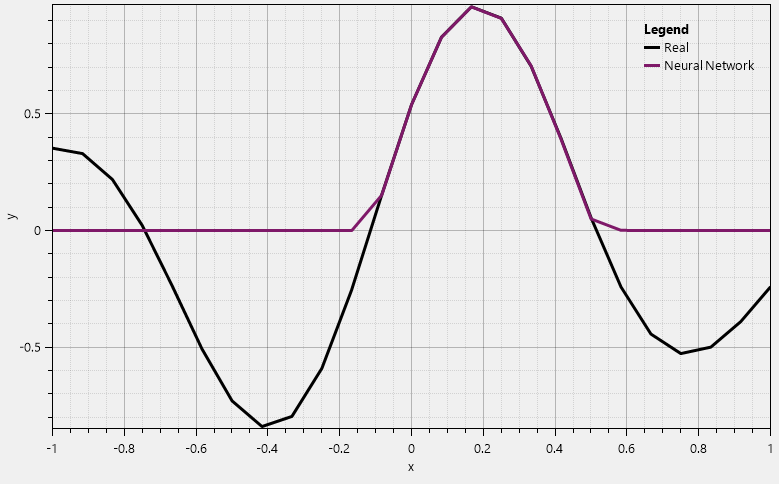
\includegraphics[width = .75\textwidth]{nn.png}
	\caption{25 points of the function $f(x) = \cos(5x-1)\exp(-x^2)$ have been plotted and fitted by minimizing the cost function of a neural network with 25 hidden nodes and a gaussian activation function.}
\end{figure}


\subsection{Splines}\label{akima}
\begin{figure}[H]
	\centering
	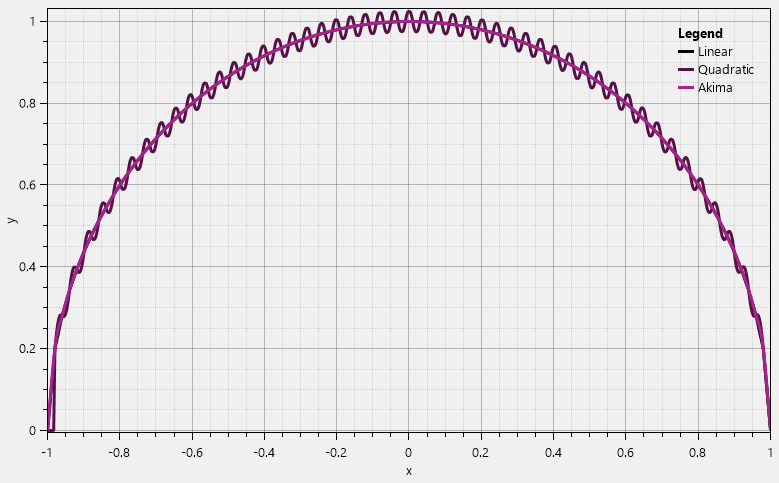
\includegraphics[width = .75\textwidth]{circleplot.png}
	\caption{Spline interpolation of different types. $N = 100$ points on the unit circle are generated. The quadratic ocelates around each point. The doubled integral from -1 to 1 evaluates to 3.1382 (linear), 3.1355 (quadratic), 3.1395 (Akima)}
\end{figure}
\subsection{Monte carlo}
Estimating pi with normal pseudo-generation: 3.14178292. And with low discrepancy (Van der Corput and Halton sequences) the estimation is: 3.14159256. Both estimations are by 100.000.000 generated numbers.


\subsection{Minimization and root-finding}
Equation 6.13 in Fedorov gives a condition for the Jacobian matrix update difference $\Delta \pmb J$:
\begin{equation}
(\pmb J + \Delta \pmb J)\Delta x = \Delta \pmb f
\end{equation}
We choose the symmetric update given by setting $\Delta \pmb J = \pmb u\pmb u^T$, and update the Jecobiann accordingly. We find the inverse with our previous matrix methods. Then $\Delta \pmb x = -\lambda \pmb  J^{-1}\pmb f(\pmb x)$, where $0<\lambda\leq 1$ is found by linesearch.\\

Likewise, equation 7.9 in Fedorov gives a condition for the hessian matrix update difference $\delta \pmb H$:
\begin{equation}
\nabla f(\pmb x+\delta \pmb x) - \nabla f(\pmb x) = (\pmb H(\pmb x) + \delta \pmb H)\delta \pmb x
\end{equation}
We choose the symmetric update given by setting $\delta \pmb H = \pmb u\pmb u^T$, and update the inverse Hessian accordingly. Then $\Delta \pmb x = -\lambda \pmb H^{-1}\nabla f(\pmb x)$, where $0<\lambda\leq 1$ is found by linesearch.
\section{References}
\begin{enumerate}
		\item \url{https://en.wikipedia.org/wiki/Givens_rotation}\\
		\item \url{https://phys.au.dk/~fedorov/Numeric/now/Book/main.pdf}
	\end{enumerate}
\end{document}